\documentclass{article}
\usepackage{listings}
\usepackage{tikz}
\usepackage[T1]{fontenc}
\usepackage{graphicx}
\usepackage{systeme}
\usepackage{fixltx2e}
\usepackage{subcaption}
\usepackage{multirow}
\usepackage{amsmath}
\usepackage{amssymb}
\let\emptyset\varnothing
\usepackage{commath}
\lstset{basicstyle=\ttfamily\footnotesize,breaklines=true}
\usepackage{float}

\title{Assignment  4\\ \vspace{0.2cm}

		COMP3670
}



\begin{document}
\setlength\parindent{0pt}
\maketitle
% \newpage
\vspace*{\fill}
    \begin{center}
    
        \textbf{name:}\author{Xuecheng Zhang}
        \\
        \textbf{UID:}u6284513
        
        \vspace{1.8cm}
        
        \date{31/8/2020}
    
    \end{center}
\vspace*{\fill}

\newpage

\textbf{Exercise 1}\\
\textbf{a)}Verify that p($\theta$)= 6$\theta$(1-$\theta$ ) is a valid probability distribution on [0, 1] (i.e. that it is always non-negative and that it is normalised.)\\
\begin{figure}[H]
\centering
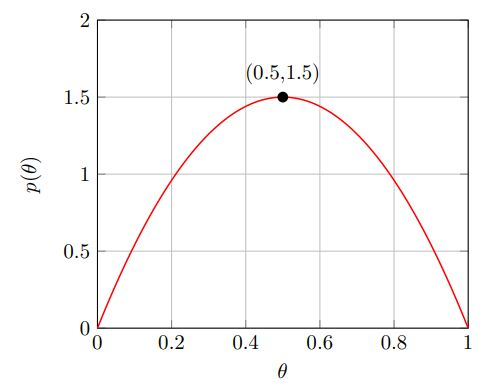
\includegraphics[width = \linewidth]{1.jpg}
\end{figure}
From the graph in the above, it can be manifest that p($\theta$) $\geq$  0, when $\theta \in [0,1]$. 
What is more, as $\int_{0}^{1} 6\theta (1-\theta ) = 1$. p($\theta$) is normalized probability.

\textbf{b)}
\[p(\theta| x_1 = 0 ) = \frac{p(x_1 = 0|\theta)\cdot p(\theta)}{p(x_1 = 0)} = \frac{6\theta(1-\theta)^2}{\int_{0}^{1}6\theta(1-\theta)^2 d\theta}= 12\theta\cdot(1-\theta)^2\]
\[p(\theta | x_{1:2} = 00) = \frac{p(x_{1:2} = 00 | \theta)\cdot p(\theta)}{p(x_{1:2} = 00)} = \frac{(1-\theta)^2\cdot 6\theta(1-\theta)}{\int_{0}^{1}(1-\theta)^2\cdot 6\theta(1-\theta)d\theta} = 20\theta(1-\theta)^3\]

c) $\mu_1$ = $\frac{1}{1-0}\int_{0}^{1} 6\theta (1-\theta)\theta d\theta = \frac{1}{2}$\\
$\mu_2$ = $\frac{1}{1-0}\int_{0}^{1} 12\theta (1-\theta)^2 \theta d\theta = \frac{2}{5}$\\
$\mu_3$ = $\frac{1}{1-0}\int_{0}^{1} 20\theta (1-\theta)^3 \theta d\theta = \frac{1}{3}$\\

d) $\sigma^2_1$  = $\int_{0}^{1} (x-\mu_1)^2 p(\theta)d\theta $ = $\frac{1}{20}$\\
$\sigma^2_1$  =$\int_{0}^{1} (x-\mu_2)^2 p(\theta)d\theta $ = $\frac{1}{25}$\\
$\sigma^2_2$ = $\int_{0}^{1} (x-\mu_3)^2 p(\theta)d\theta $ = $\frac{2}{63}$

\begin{table}[]
\centering
\begin{tabular}{|l|l|l|l|l|}

\hline
\textbf{Posterior} & \textbf{PDF} & \textbf{$\mu$} & \textbf{$\sigma^2$} & \textbf{$\theta_{MAP}$} \\ 
\hline
      $p(\theta)$ &  6$\theta$(1-$\theta$)& $\frac{1}{2}$ & $\frac{1}{20}$ & $\frac{1}{2}$ \\
       \hline
      $p(\theta|x_1 = 0)$ & $12\theta\cdot(1-\theta)^2$ & $\frac{2}{5}$ & $\frac{1}{25}$ & $\frac{1}{3}$ \\ 
      \hline
      $p(\theta|x_{1,2} = 00)$ & $20\theta(1-\theta)^3$ & $\frac{1}{3}$ &  $\frac{2}{63}$ &  $\frac{1}{4}$\\
       \hline
\end{tabular}
\end{table}
\textbf{f. Plot each of the probability distribution $p(\theta)$, p($\theta|x_1 = 0$), p($\theta|x_{1:2} =00 $) over the interval 0 $\leq$ $\theta$ $\leq$ 1 on the same graph to compare them.} \\
Let $f(1) = p(\theta)$, $f(2) = p(\theta|x_1 = 0)$, $f(3) = p(\theta | x_{1:2} = 00)$. 
\begin{figure}[H]
\centering
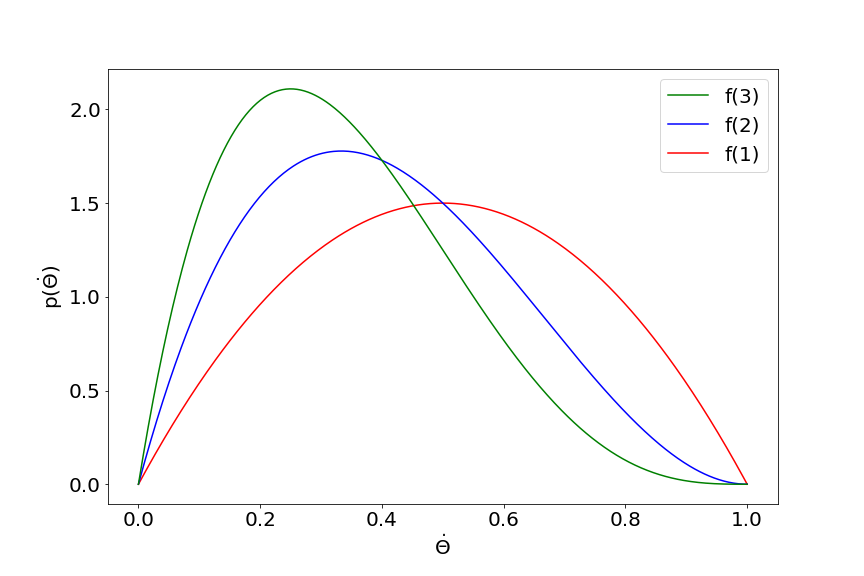
\includegraphics[width = \linewidth]{1.png}
\end{figure}
f(3) has the maximum value among f(2) and f(1). Also, it is faster than others approaching to the maximum value and its increase rate is higher than f(2) and f(1). However, the decrease rate is slower than f(2) and f(1).\\

\textbf{g. What behaviour would you expect of the posterior distribution p($\theta|x_1:n$) if we updated on a very long sequence of alternating coin flips $x_1$:n = 101010101 $\cdots$}\\
\[
p(\theta|x_1:n = 0101010\cdots) = \frac{6\theta^{1+\frac{n}{2}}(1-\theta)^{1+\frac{n}{2}}}{\int_0^{1}{6\theta^{1+\frac{n}{2}}(1-\theta)^{1+\frac{n}{2}}}d\theta}
\]

I plot several values for different n value:\\

\begin{figure}[H]
\centering
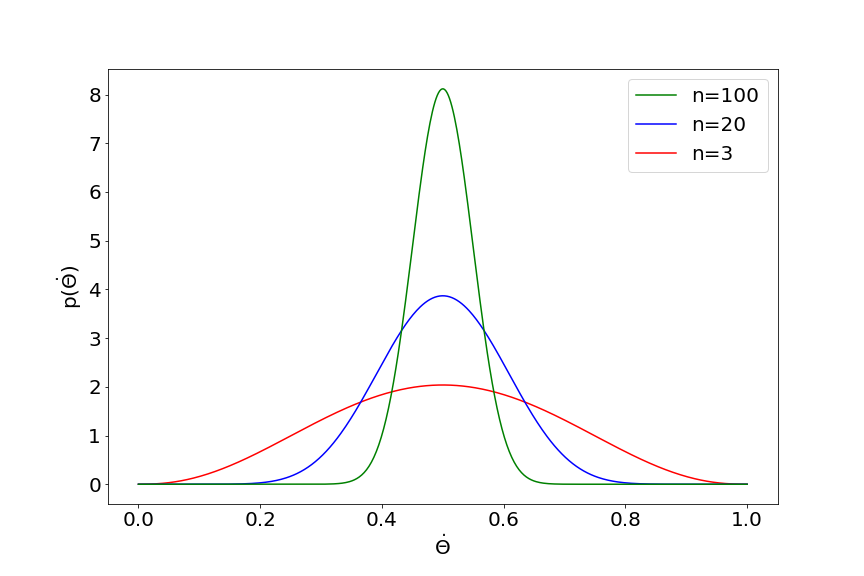
\includegraphics[width = \linewidth]{2.png}
\end{figure}

From the above graph, I observe that the graph is squeezed to the center and the line of the graph is more steeper for bigger n value. What is more, the maximum value of function is increasing dramatically with bigger n value. \\

When n is sufficiently large, the maximum value will approach to the infinity and the function will be completely squeezed to the center.\\\textbf{(Let f(4) = p($x_1$:n = 101010101 $\cdots$) )}
\begin{figure}[H]
\centering
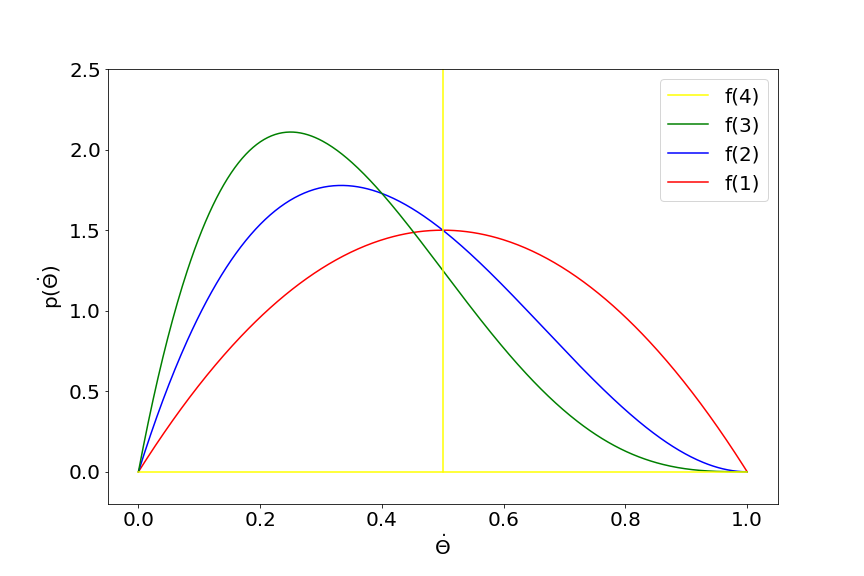
\includegraphics[width = \linewidth,height = 210px]{3.png}
\end{figure}

As the probability of 1 and 0 is the same when n is sufficiently large, the expected value \textbf{$\mu$} is $\frac{1}{2}$. The  variance of function is 0 as most areas of the function is flat,i.e. $\sigma^2 = 0$ The function has the maximum value when $\theta = \frac{1}{2}$, i.e. \textbf{$\theta_{MAP} = \frac{1}{2}$ }\\

\textbf{Question 2:}\\
\textbf{a.  Briefly comment about how the camera behaves for $\phi$ = 0,$\phi$ = 0.5,$\phi$ = 1. How you
expect this would change how the agent updates it’s prior to a posterior on $\theta$, given an observation of $\hat{X}$.}\\
If $\phi$ =0, whenever the obverse of coin is 1 or not, the agent can only observe 0. There is no evidence add to the posterior since the observation remains the same. Therefore, \textbf{the posterior is updated to the same value as prior.}\\
If $\phi$ =0.5, when the obverse of coin is 1, the agent has half of possibility to get the correct answer. It generates some new information because the observation of the coin depends on the probability. Therefore, \textbf{the posterior is updated to the value different from prior.}\\
If $\phi$ = 1, the agent can correctly get all the answer. There is no evidence add to the posterior since the observation always provide the correct result of the coin. The observation is mainly effect by the probability of coin flip.Therefore, \textbf{the posterior is updated to the same value as prior.} \\

\textbf{b. Compute p($\hat{X} = x|\theta, \phi$) for all x $\in$ {0,1}.}\\
When x = 0 $\in$ \{0,1\}:
\begin{gather}
p(\hat{X} = 0|\theta, \phi) = \sum_x{p(\hat{X} = 0, X = x|\theta, \phi) } \notag \\ \notag = \sum_x{p(\hat{X} = 0|X= x,\theta,\phi)p(X=x|\theta,\phi)}
\end{gather}
As the real coin probability does not depend on $\phi$, $p(X=x|\theta,\phi)$ can rewritten as $p(X=x|\theta)$. What is more, when we know the result of coin flip, $\theta$ does not have affect on it. \\

The formula can be rewritten as:\\
\begin{gather}
\sum_x{p(\hat{X} = 0|X= x,\phi)p(X=x|\theta)} \notag \\
= p(\hat{X} = 0 | X = 0,\phi)p(X = 0| \theta) + p(\hat{X} = 0 | X = 1,\phi)p(X = 1| \theta) \notag \\
= 1 \cdot (1-\theta) + (1-\phi) \cdot \theta
\end{gather}

When x = 1 $\in$ \{0,1\}:
\begin{gather}
p(\hat{X} = 0|\theta, \phi) = \sum_x{p(\hat{X} = 0, X = x|\theta, \phi) } \notag \\ \notag = \sum_x{p(\hat{X} = 0|X= x,\theta,\phi)p(X=x|\theta,\phi)} \\
= \sum_x {p(\hat{X} = 1| X =x,\phi) p(X= x|\theta)} \notag\\ = p(\hat{X} = 1 | X = 0,\phi)p(X = 0| \theta) + p(\hat{X} = 1 | X = 1,\phi)p(X = 1| \theta) \notag \\ 
= 0 + \phi \cdot \theta =  \phi \theta
\end{gather}

In conclusion, x= 0, $p(\hat{X} = 0|\theta, \phi) = 1 - \phi \theta$. x = 1, $p(\hat{X} = 1|\theta, \phi) =\phi \theta$\\

\textbf{c. What term does p($\theta|\hat{x_1} = 0,\phi$) simplify to when $\phi$ = 1? When $\phi$ = 0? Explain your observations.}\\
\begin{gather}
p(\theta|\hat{x_1} = 0,\phi)=\frac{p(\hat{x_1} =0|\theta,\phi) p(\theta|\phi)}{p(\hat{x_1} = 0|\phi)} \notag\\
= \frac{p(\hat{x_1} =0|\theta,\phi) p(\theta|\phi)}{\int_0^1{p(\hat{x_1} =0|\theta,\phi) p(\theta|\phi)}d\theta} = \frac{(1-\phi \theta)\cdot 6\theta \cdot(1-\theta)}{\int_0^1 (1-\phi \theta)\cdot 6\theta \cdot(1-\theta) d\theta} \notag \\ = \frac{(1-\phi\theta)\cdot 12\theta (1-\theta)}{2-\phi}
\end{gather}

When $\phi = 0$, \[ p(\theta|\hat{x_1} =0,\phi)  = 6\theta(1-\theta) = P(\theta|\phi = 0) = P(\theta|0). \]  The posterior probability is equal to the prior probability. As $\hat{X}$ always equal to 0, the result of agent observation is meaningless. After the prior probability, it does not add any additional information thus the posterior probability is still equal to the prior probability. \\
The term is simplified as $p(\theta)$ from Question 1. As the observation of $\hat{x_1}$ does not have an effect of $p(\theta)$(since it always equals to 0.) and $\theta$, $\phi$ are independent, P($\theta|0$) = P($\theta$) \\

When $\phi = 1$, \[ p(\theta|\hat{x_1} =0,\phi) = 12\theta(1-\theta)^2 = P(\theta|\phi = 1)  = P(\theta|1). \] The posterior probability is equal to the prior probability. No additional information is added to the posterior probability. As $\phi = 1$, the probability which the camera observes is basically the same as the coin flip. Furthermore, $\phi$, $\theta$ are independent. Therefore, the term can be simplified as $p(\theta|\hat{x_1} =0,\phi) = p(\theta|x_1 = 0)$ \\

\textbf{d. Comment on how the result depends on $\phi$. Does the result make sense?}
\begin{gather}
p(\theta|\hat{x_1} = 1,\phi)=\frac{p(\hat{x_1} =1|\theta,\phi) p(\theta|\phi)}{p(\hat{x_1} = 0|\phi)} \notag\\
= \frac{p(\hat{x_1} =1|\theta,\phi) p(\theta|\phi)}{\int_0^1{p(\hat{x_1} =1|\theta,\phi) p(\theta|\phi)}d\theta} = \frac{(\phi \theta)\cdot 6\theta \cdot(1-\theta)}{\int_0^1 (\phi \theta)\cdot 6\theta \cdot(1-\theta) d\theta} \notag \\ = \frac{(\phi\theta)\cdot 12\theta (1-\theta)}{\phi} = 12 \theta^2 \cdot(1-\theta)
\end{gather}

When $\phi = 0$, \[ p(\theta|\hat{x_1} =1,\phi)  =  12 \theta^2 \cdot(1-\theta). \]  

When $\phi = 1$, \[ p(\theta|\hat{x_1} =1,\phi) =  12 \theta^2 \cdot(1-\theta) \]

\textbf{The result of p($\theta|\hat{x_1} = 1,\phi$) is not related to $\phi$ so that they are independent.} In the probability $p(\theta|\hat{x_1} =1,\phi)$, the $\phi$ does not effect on the $\theta$ value. The formula can be rewritten as $p(\theta|\hat{x_1} =1)$. What is more, only if $x_1$ is equal to 1, the value of $\hat{x_1}$ is 1. The principle of getting $\hat{x_1} = 1$ is only related to $\theta$ since it does not depend on the the camera. Therefore, $\phi$ does not effect on the p($\theta|\hat{x_1} = 1,\phi$)\\

\textbf{e. Comment on how the shape of the distribution }
\begin{figure}[H]
\centering
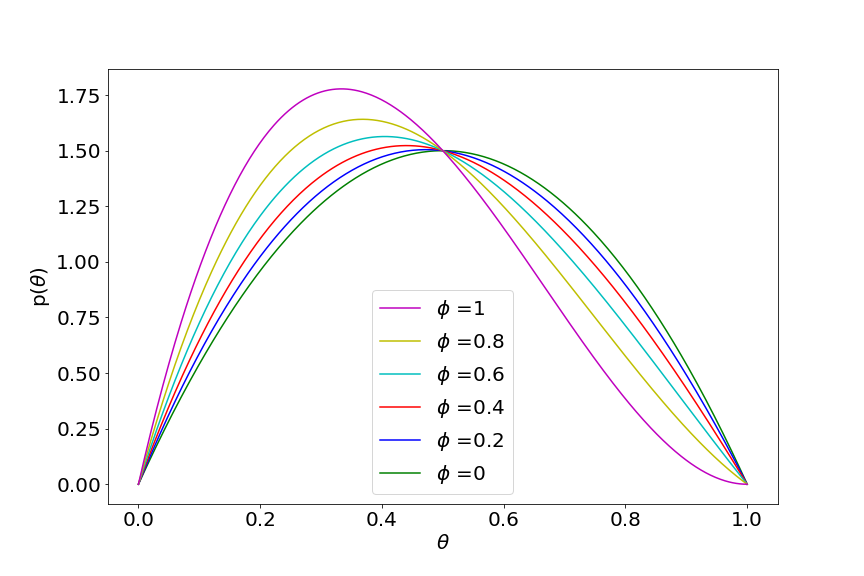
\includegraphics[width = \linewidth]{4.png}
\end{figure}
As $\phi$ increases, the image tilts to the left and the gravity center of the graph shifted to the left. The maximum value of the graph is increases when $\phi$ increases. When $\phi$ increases, the probability of obtaining the correct value increase. When $\phi$ increases, the camera will make fewer mistakes, the probability of observing $\hat{x} = 0$ increases as the probability of correctness increases. When $\phi$ equal to 0, the probability of observing $\hat{x} =0$ has the least probability. \\

\textbf{Question 3:}\\
We compute the CDF function of Y,\\
Since x $\in$ [0,1]:\\
$F_Y(y)$ = P(Y $\leq$ y) = P($X^2+1 \leq$ y) = P($|X| \leq$ $\sqrt{y-1}$)  \\= $\int_{0}^{\sqrt{y-1}} 2-2x dx$ = $2\sqrt{y-1}-y+1$\\
We can obtain the pdf Y by differentiating:
p(y) = $\frac{d(2\sqrt{y-1}-y+1)}{dy}$ = $\frac{1}{\sqrt{y-1}}-1$\\



\newpage
\textbf{Discussion:}\\
Have a discussion with u6548263 on Question 2 part b and c.

\end{document}

